The Silicon Photomultiplier (SiPM) are a kind of photosensor, based on semiconductor materials, developed in recent years. They are replacing progresively conventional PMTs in many experiments and applications. They archieve outstading photon-counting capabilities with high photodetection efficiency comparing to PMT and similar gain. They have conveninent characteristics as insensitiveness to magnetic fields, low operating voltage and compactness. The main problem with the SiPMs are their high dark count rate (between $100~\kilo\hertz$ and $1~\mega\hertz$).

The SiPM is formed by a matrix of APDs conected in parallel which are photodiodes operating in Geiger mode. APDs, the scheme of which is shown in Figure \ref{fig:SchemeAPD}, are based on p-n junctions\footnote{A p-n junction is a junction of a p+ and n+ layer, which are a tetravalent material doped with a trivalent or pentavalent material respectively, creating interesting sublevels in the forbidden energy gap.} made with special techniques to archieve a good contact between both surfaces.

\begin{figure}[htbp]
\centering
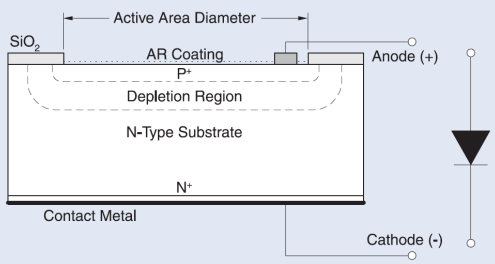
\includegraphics[scale=0.6]{3DesignPrinciples/32Tritium_detector/APD_scheme.png}
\caption{Scheme of a APD and electrical symbol used.\label{fig:SchemeAPD}~\cite{OSI}}
\end{figure}
 

The voltage at which the SiPM starts operating in geiger mode is called the breakdown voltage, $V_ {BD}$. At lower voltages SiPM works in proportional mode in which the signal of the pixel is proportional to the energy deposited but its gain is lower than in Geiger mode. The experimental measurement of the breakdown voltage, described in section \ref{sec:CharacterizationSiPM}, is an important measurement to characterize a SiPM since many properties of the SiPM depends on the overvoltage, $V_{ov}$. The overvoltage is the voltage applied to the SiPM above their own breakdown voltage and this is expressed as:

\begin{equation}
V_{bias}=V_{BD}+V_{OV}
\label{overvoltage}
\end{equation}

These APDs, called pixels when they are part of a SiPM, are connected in parallel and the sum of all of them is read. The output signal of an individual pixel is quite similar regardless of the energy deposited, with some difference because of the uncertainty due to the SiPM manufacturing process and the statistical nature of the detection process. Therefore, the energy deposited in each APD is not known but the charge of the output signal when n pixels are simultaneously fired is n times the charge of a single pixel, as can be checked in Figure \ref{fig:PulsesOfSiPM}. Due to this property, considering that each pixel only detect one photon, the number of detected photons is linearly proportional to the area of the output signal. Hence, after a correct calibration of SiPMs, shown in section \ref{sec:CharacterizationSiPM}, the linearity of the SiPM output signal and the deposited energy by the tritium event is recovered.

\begin{figure}[h]
\centering
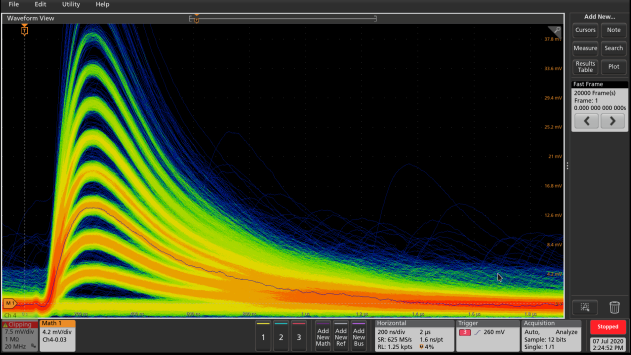
\includegraphics[scale=0.6]{3DesignPrinciples/32Tritium_detector/Several_SiPM_pulses.png}
\caption{SiPM output pulses displayed on oscilloscope, model MSO44X from Tektronix \cite{Oscilloscope}. To easily observe several heights of these pulses, associated with a different number of  SiPM pixels fired at the same time, the persistence function of the oscilloscope is used.\label{fig:PulsesOfSiPM}}
\end{figure}

The size of a SiPM pixel has to be very small\footnote{Pixel sizes for commercial SiPMs are $25$, $50$ or $75\mu\meter$ \cite{DataSheetHammamatsu_1_SiPM_25}, \cite{DataSheetHammamatsu_1_SiPM_50}, \cite{DataSheetHammamatsu_1_SiPM_75}} to make sure that, for low enough photon densities to be detected, only one photon is detected in each pixel. If the photon density is high (typically several thousand of photons per event) more than one photon will be detected by the same pixel, generating an output signal equal to one detected photon. This effect, known as saturation, produces a loss of linearity of the output signal. However, this effect is not important for the TRITIUM detector since its scintillating signals are futher away from producing it. %The experimental measurements of this effect, which have been done for our SiPMs, is shown in section \ref{sec:CharacterizationSiPM}. 

The SiPM can be modeled as the electric circuit, shown in figure \ref{subfig:ElectricModelSiPM}, in which, due to the charge distribution in the depletion zone, a capacitance are induced by the SiPM. This looks like as a reverse diode in parallel with a capacitor with a capacitance of $C_d$. When the pixel detects a photon, the capacitor are discharged, creating an output current (electronic pulse).

In addition, each pixel of a SiPM has a quenching resistance\footnote{The tipical valuer of this quenching resistance for commercial SiPMs is around $500~\kilo\Omega$}, $R_q$, in series that is used to stop the current produced when this pixel is fired. When the discharge is produced, a current flow throguth the resistance, reducing the reverse voltage seen by the diode to one below the breakdown voltage. Then, the current that flow throught the diode is stopped and the voltage seen by the diode is reset to the bias voltage. This pixel is ready to detect a new photon again. This behaviour is schematicaly shown in Figure \ref{subfig:HowSiPMworks}.

\begin{figure}
\centering
    \begin{subfigure}[b]{0.45\textwidth}
    \centering
    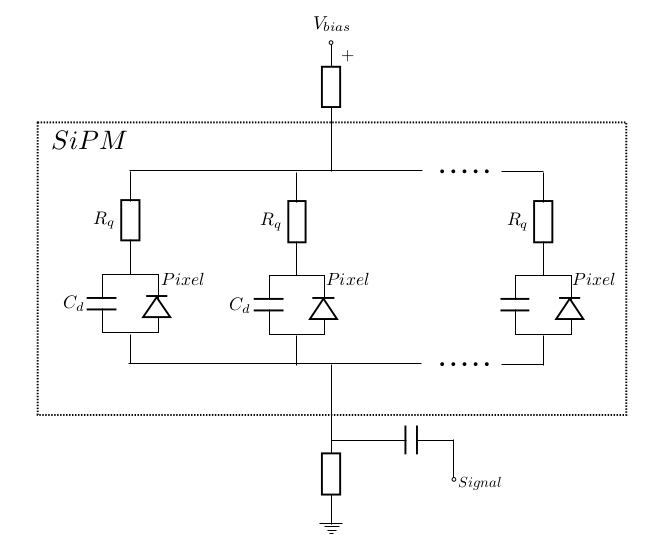
\includegraphics[width=\textwidth]{3DesignPrinciples/32Tritium_detector/SimpliestElectronicSchemeSiPM.png}  
    \caption{Photon Detection Efficiency, PDE.\label{subfig:ElectricModelSiPM}}
    \end{subfigure}
    \hfill
    \begin{subfigure}[b]{0.45\textwidth}
    \centering
    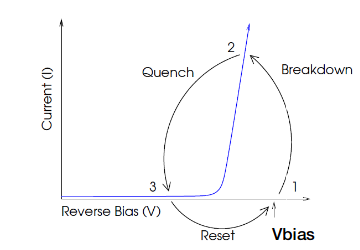
\includegraphics[width=\textwidth]{3DesignPrinciples/32Tritium_detector/How_a_quenching_resistence_in_a_SiPM_works.png}  
    \caption{Output current of a SiPM.\label{subfig:HowSiPMworks}}
    \end{subfigure}
 \caption{(Left) Electronic scheme of a SiPM and (right) output current of a SiPM as a function of the reverse voltage. It show that the quenching mechanism is essential for working with SiPMs~\cite{DataSheetSensL}.}
 \label{fig:ChenchingResistance}
\end{figure}

The recovery of the bias voltage seen by the SiPM after a photon detection is that characteristic in a RC circuit, described by the equation: 

\begin{equation}
V_{bias}(t)=V(t_0)\left(1-e^{-t/\tau} \right)
\label{RCCircuitBiasVoltage}
\end{equation}
where $\tau$ is the recovery time constant of the system, the value of which is $\tau=C_d \times R_q$ for RC circuits.

In section \ref{sec:CharacterizationSiPM} the capacitance $C_d$ and the quenching resistance $R_q$ are experimentally measured and the recovery time constant extrapolated from both.

SiPM gain is defined as the charge produced when a single pixel is fired. This can be measured experimentally from its Single Photon Spectrum, SPS, which is the spectrum obtained when the SiPM output signal is integred (charge) and histogrammed. The SiPM gain is typically of the order of $10^6$. The experimental measurement of the SPS and the calculation of the gain is presented in section \ref{sec:CharacterizationSiPM}.

It has to be taken into account that the SiPM gain is highly dependent on temperature, which cannot be controlled with sufficient sensitivity (less than $1\celsius$) in the final emplacement of the TRITIUM monitor. Therefore, a gain stabilization method was developed to compensate for the temperature effect. This method is detailed and tested in section \ref{sec:CharacterizationSiPM}.

Other important parameter for a SiPM used in the TRITIUM project is de photon detection efficiency, PDE. This is defined as the probability of recording the electrical pulse produced by a photon that hit the SiPM. The PDE of a SiPM consists of a product of three different paramenters, the fill factor ($FF$), which is the ratio between the active area of the SiPM and the total area, the quantum efficiency for photoelectron conversion ($QE$), which is the probability that a incident photon generate an electron-hole pair, and the probability that the generated electron or hole produces an avalanche, $P_{av}$.

\begin{equation}
PDE=FF \times QE \times P_{av}
\label{PDE_SiPM}
\end{equation}

Like PMTs, sometimes the SiPM produces pulses that are unrelated with any incident photon, called dark current rate. The dark current rate depends on the temperature and, at temperatures around $25\celsius$, these pulses are mainly produced by the thermal generation, which is produced when a free electron or hole start an avalanche. This signal is identical to the signal produced due to a detection of a single photon so they cannot be differentiated. Therefore, it is very important to determinate their importance on the tritium signal.

Electrons contained in an avalanche of a SiPM pixel emit secondary optical photons\footnote{Around 20 secondary optical photons are emitted for SiPMs with gains of the order of $10^6$ \cite{CrosstalkProbability}}. These optical photons can reach other pixels, producing new avalanches. This effect, called optical crosstalk, produces signals that are larger than those corresponding to the detected event, producing erroneous information about the number of photons read. The probability of producing an optical crosstalk event depends on the number of electrons produced in the avalanche (gain) and, therefore, depends on the temperature and the overvoltage. This is typically less than $10\%$ at the recommended overvoltage and temperatures around $25\celsius$.

The PED, dark count rate and Crosstalk are not experimentaly measured yet since a different setup, shown in reference \cite{PDEStudy}, is needed. These parameters will be measured for the SiPM model used in the final version of TRITIUM monitor.

Due to imperfections existing in the cristal lattice of a SiPM, called traps, an electron of an avalanche can be captured and released after a characteristic time, $\tau_t$. If this characteristic time is longer than the time used to recover the charge of the pixel, typically $3\tau$, this electron can trigger a new avalanche which will be seen as a new event. This events, called  afterpulses, are often emitted around $1~\mu\second$s after some SiPM output pulses. The afterpulse probability was not measured since they are not interesting. The reason is that the TRITIUM detecter use the SiPM as a counter (without integring the signal). In addition, PETSYS make time coincidences using time time windows of $10~\nano\second$. At this level the afterpulse probability is negligible since it normally happen $1~\mu\second$ after the SiPM output pulse.

The initial cadidate for TRITIUM project and the one which was characterized is the model S13360-1375 from Hamamatsu Photonics \cite{DataSheetHammamatsu_1_SiPM_1375} because this has interesting characteristics and properties, shown in Table \ref{tab:PropertiesOfSiPM1375}. This model was mainly choosen due to its large pixel size, $75~\mu\meter$, which implies high PDE and high gain, both parameters are important for the TRITIUM project due to the low activity to be detected and the small signals produced by tritium events, respectively. This is achieved at the cost of reducing the dinamic range, which is not a problem due to the small signal generated by tritium events. 

\begin{table}[h]
%%\centering.
\begin{center}
\begin{tabular}{|c|c|c|}
\hline
Parameter & S13360-1375 & S13360-6075 \\
\hline \hline \hline
Serie & $S13360$ & $S13360$ \\ \hline
Model & $1375$ & $16075$ \\ \hline
Pixel Pitch ($\mu\meter$) & $75$ & $75$ \\ \hline
Effective photosensitive area ($\mm^2$) & $1.3 \times 1.3$ & $6.0 \times 6.0$ \\ \hline
Number of pixels & $285$ & $6400$ \\ \hline
Fill factor & $82\%$ & $82\%$ \\ \hline
Refractive index of windows material & $1.55$ & $1.55$ \\ \hline
Operating temperature range ($\celsius$) & $[-20,60]$ & $[-20,60]$ \\ \hline
Spectral response range, $\lambda$ ($\nano\meter$) & $[320, 900]$ & $[320, 900]$ \\ \hline
Peak sensitivity wavelength, $\lambda_p$ ($\nano\meter$) & $450$ & $450$ \\ \hline
PhotoDetection Efficiency, PDE, $\lambda=\lambda_p$ ($\%$) & $50$ & $50$ \\ \hline
Dark counts, Typical/Maximum (kcps) & $90/270$ & $2000/6000$ \\ \hline
Terminal capacitance, $C_t$ ($\pico\farad$) & $60$ & $1280$ \\ \hline
Gain, M, & $4 \cdot{} 10^6$ & $4 \cdot{} 10^6$ \\ \hline
Breakdown Voltage, $V_{BD}$ ($\volt$) & $50,97$ & $53$ \\ \hline
Cross talk probability($\%$) & $7$ & $7$ \\ \hline
Temperature coefficient $\Delta TV_{op}$ (m$\volt/\celsius$) & $54$ & $54$ \\ \hline
\end{tabular}
\caption{Characteristics of SiPM S13360-1375 from Hamamatsu Photonics \cite{DataSheetHammamatsu_1_SiPM_1375}.}
\label{tab:PropertiesOfSiPM1375}
\end{center}
\end{table}

These values, provided by Hamamatsu photonics, are only approximate for a given element. Therefore, these parameters must be experimentally measured for each SiPM used because they can vary significatively even for SiPMs of the same model. Some most important characteristics for the TRITIUM project are experimentaly measured and given in section \ref{sec:CharacterizationSiPM}. 

This model was also chosen because, as can be seen in Figure \ref{fig:PDESiPM}, its maximum PDE is reached at $\lambda_p=450~\nano\meter$, which is very close to the peak of the emission spectrum of the scintillating fibers used, $\lambda_e=435~\nano\meter$.

\begin{figure}[htbp]
\centering
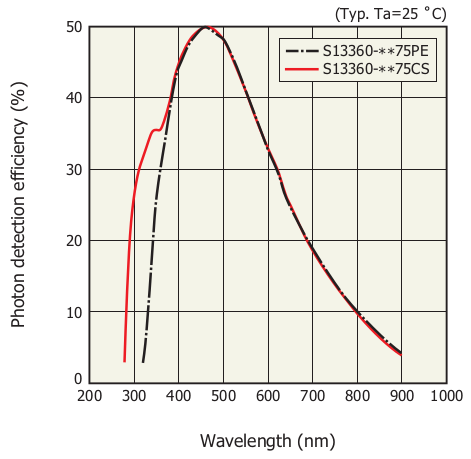
\includegraphics[scale=0.6]{3DesignPrinciples/32Tritium_detector/SiPMPDE.png}
\caption{Photon detection efficiency (PDE) spectrum of SiPM S13360-**75 models.\label{fig:PDESiPM}}
\end{figure}

This model was later replaced by the model S13360-6075 from Hamamatsu Photonics \cite{DataSheetHammamatsu_1_SiPM_75}. The only difference between both is its higher active area ($6\times6~\mm^2$) with which larger active area of scintillating fibers can be read. This improvement is achieved at the price of a higher dark count rate (typically 2 Mcps). In addition, commercial matrices are available, covering a total size of $24\times24~\mm^2$.

Although TRITIUM detector uses whole SiPM matrices, the caracterization has been carried out first at the level of a single SiPM to learn about the values of the SiPM parameters and to test the gain control method. A new experimental setup, detailed in appendix \ref{App:ElectronicReadoutSiPM}, is already  prepared to perform a complete characterization of the SiPM model S13360-6075.